% ---------------------------------------------------------------------------------------
\chapter{Análisis y Procesamiento de Imagenes }\label{chap5}

\section{Introducci\'on}

Tanto en la ciencia de datos, commom en estad\'istica, y la compitaci\'on, el an\'alisis de im\'agenes es un ha emergido como un \'area de estudio de gran importancia, que he sido pivotal y con un extenso alcance en multiples discuplinas. De la forma en que la era digital avanza, la cantidad de datos que se generan en forma de im\'agenes es cada vez mayor, y con ello la necesidad herramientas para analizar, procesar, comprender y en general obtener informaci\'on relevante de estas imagenes. 

El uso de im\'agenes ha evolucionado de aplicaci\'ones tradicionales como imagenolog\'ia satelital y diagn\'ostico m\'edico, a dominios m\'as modernos como inteligencia artificial, reconocimiento facial, y vehiculos aut\'onomos. La habilidad de detectar patrones, animal\'ias, y derivar informaci\'on de estas tiene un potencial enorme para la innovaci\'on y el desarrollo de nuevas tecnolog\'ias. 

En este cap\'itulo, se introducen los conceptos necesarios para entender el an\'alisis de im\'agenes, y se presentan las herramientas que se utilizaron para el desarrollo de este trabajo. Comenzaremos defininiendo las imagenes como matrices, luego presentaremos el banco de imagenes a utilizar durante el resto del trabajo, para posteriormente hablar de las caracter\'isticas de una imagen, como el contraste, la luminosidad, y la saturaci\'on. Luego, hablaremos de los espacios de color, y como estos se utilizan para representar una imagen. Finalmente, hablaremos de las t\'ecnicas de comparaci\'on de im\'agenes, en particular como aplicamos t\'ecnicas de comparaci\'on entre vectores sobre im\'agenes,

% ---------------------------------------------------------------------------------------
\section{Imagenes como matrices}

Una im\'agen es una representaci\'on visual de un objeto, y se puede definir como una funci\'on bidimensional $f(x,y)$, donde $x$ y $y$ son coordenadas espaciales, y el valor de $f$ en cualquier par de coordenadas $(x,y)$ es la intensidad de la imagen en ese punto. Cuando $x$, $y$, y los valores de intensidad de $f$ son todos finitos y discretos, llamamos a la imagen una imagen digital. En este trabajo hemos utilizado (y seguiremos utilziando) el concepto de imagen digital e im\'agen de forma intercambiable. Por claridad en notaci\'on y conveniencia, usamos valores enteros para determinar las coordenadas de la imagen, y su origen en la esquina superior izquierda, como se muestra en la siguiente ecuaci\'on:

$$
f(x, y)=\left[\begin{array}{cccc}
f(0,0) & f(0,1) & \cdots & f(0, N-1) \\
f(1,0) & f(1,1) & \cdots & f(1, N-1) \\
\vdots & \vdots & & \vdots \\
f(M-1,0) & f(M-1,1) & \cdots & f(M-1, N-1)
\end{array}\right]
$$

El lado derecho de esta ecuación es una imagen digital representada como un conjunto de números reales. Cada elemento de este conjunto se llama elemento de imagen, píxel o "pel". La Figura \ref{fig:dip_2_18} muestra una representación gráfica de un conjunto de imágenes, donde los ejes $x$ e $y$ se utilizan para denotar las filas y columnas del conjunto. Píxeles específicos son valores del conjunto en un par fijo de coordenadas. Como se mencionó anteriormente, generalmente utilizamos $f(i, j)$ al referirnos a un píxel con coordenadas $(i, j)$.


\begin{figure}[H]
    \centering
    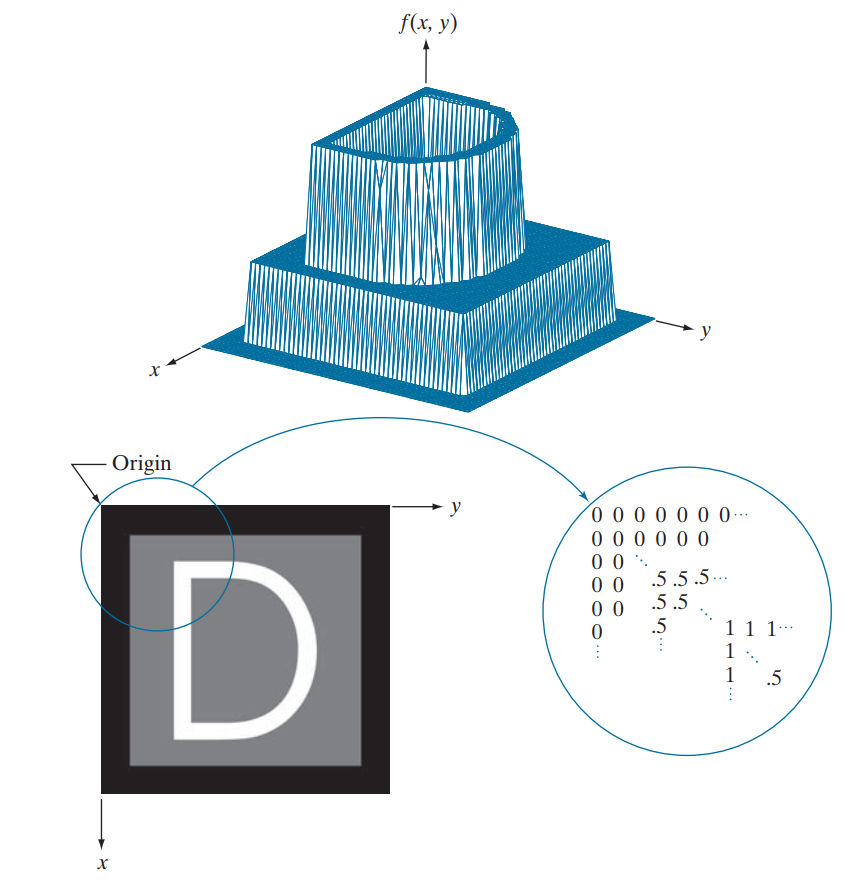
\includegraphics[width=0.5\textwidth]{dip_4_fig2_18.png}
    \caption{
        (a) Imagen representada como una superficie.
        (b) Imagen mostrada como un conjunto de intensidades visuales.
        (c) Imagen presentada como un conjunto numérico en 2D. (Los números 0, 0.5 y 1 representan negro, gris y blanco, respectivamente).}
    \label{fig:dip_2_18}
\end{figure}

Como se ve en la figura \ref{fig:dip_2_18}, y como mencionamos anteriormente, el origen se define en la esquina superior izquierda, esta es una convenci\'on que nace en que mucha tecnolog\'ia usada para representar imagenes hacen un barrido de imagen de arriba hacía abajo y de izquierda a derecha, por ejemplo, los televisores. Esto tambi\'en es conveniente dado que concorda con la forma en la que solemos indexar matrices, las cuales tambi\'en podemos podemos utilizar para representar una imagen  de la siguiente forma:

$$
\mathbf{A}=\left[\begin{array}{cccc}
a_{0,0} & a_{0,1} & \cdots & a_{0, N-1} \\
a_{1,0} & a_{1,1} & \cdots & a_{1, N-1} \\
\vdots & \vdots & & \vdots \\
a_{M-1,0} & a_{M-1,1} & \cdots & a_{M-1, N-1}
\end{array}\right]
$$

Normalmente, cuando trabajamos con una im\'agen obtenida de una c\'amara digital, esta se encuentra en el espacio de color RGB, donde cada pixel de la imagen es representado por tres valores, uno para cada canal de color. Por tanto, podemos representar una imagen RGB como una matriz de $N \times M \times 3$, donde $N$ y $M$ son el ancho y alto de la imagen, y el tercer valor representa los tres canales de color de la siguiente forma:

$$
\mathcal{F}(x, y)=\{R(x, y), G(x, y), B(x, y)\}
$$


Con $R$, $G$, y $B$ representando los valores de los canales rojo, verde y azul respectivamente, y con $x\in[0,M-1]$ e $y\in[0,N-1]$ representando las coordenadas de la imagen. El espacio de color RGB es el espacio m\'as comun para representar imagenes en monitores y es como la gran mayoría de c\'amaras digitales capturan imagenes, pero no es el \'unico espacio de color que existe, otros ejemplos notables son el espacio CMY (cyan, magenta, yellow) y CMYK (cyan, magenta, yellow, black) son espacios comunmente utilizados en impresi\'on, y el espacio HSI (hue, saturation, intensity), que corresponde de forma cercana a la forma en la que los humanos describimos e interpretamos el color. \cite{DigitalImageProcessing}

Al momento de trabajar con imagenes para el contexto de este trabajo, nos es de interes hacerlo con imagenes en escala de grises, puesto que queremos mantener la informaci\'on espacial de la imagen, y nos facilitar\'a el calculo m\'as adelante. El paso a escala de grises no es más que un promedio ponderado de los tres canales de color de la imagen, aunque tendría sentido utilizar un promedio simple, la percepción humana varía dependiendo del color, dado que somos mas sensibles a los colores verdes, y menos sensibles a los colores azules. Para esto, podemos convertir una imagen RGB a escala de grises utilizando la siguiente ecuaci\'on:

\begin{equation}
    I(x, y)=0.299 R(x, y)+0.587 G(x, y)+0.114 B(x, y), 
    \label{eq:grayscale}
\end{equation}

que corresponde el canal gris del espacio de colores $YC_bC_r$. En la siguiente figura podemos ver una imagen RGB, una transformaci\'on utilizando un promdeio simple, y su correspondiente imagen en escala de grises como fue definida anteriormente.

% \begin{figure}
%     \centering
%     \includegraphics[width=0.5\textwidth]{rgb2gray.png}
%     \caption{Imagen RGB, promedio simple, y escala de grises.}
%     \label{fig:rgb2gray}
% \end{figure}

\todo[]{insertar imagen rgb2gray}

En la siguiente secci\'ion presentaremos el banco de imagenes que utilizamos para el desarrollo de este trabajo, y mostraremos como se ven las imagenes en escala de grises.


\section{Banco de im\'agenes}

El banco que utilizaremos es llamado \textit{Kodak Lossless True Color Image Suite
}\cite{KodakLosslessTrueColorImageSuite} que corresponde a 24 imagenes no comprimidas y con color completo. Est\'as fueron publicadas por la compa\~nia Eastman Kodak en 1999, y son ampliamente utilizadas en el \'area de procesamiento de im\'agenes. 

Podemos ver las imagenes en la figura , y podemos ver las imagenes en escala de grises en la figura 

\todo{insertar imagenes del banco de imagenes}

Est\'as imagenes correponden a una gran variedad de escenas y texturas, teniendo figuras humanas, arquitecura, y paisajes; lo que nos entrega un amplio abanico de posibilidades y variedad al momento de hacer los experimentos.

\section{Characteristicas de una imagen, y escala de grises.}


Estadistico
\todo{hablar del banco de imagenes kodak lossless true color image suite}

\section{Comparando imagenes}

\todo{secci\'on sobre como aplicamos los coeficientes de comparacion obre imagenes}
\todo{comparaci\'on entre histogramas inspirado en bicego \cite{bicego2016}}


